\chapter{Simulations}
This chapter presents the results obtained by simulations. The research has been made for two models
described in chapter \ref{ch:model}. The motion planning problem has been solved using endogenous
configuration space approach presented in chapter \ref{ch:endogen}.
\section{RobRex}
\subsection{Problem formulation}
The problem to be solved is to move the platform from the initial state
$q_0 = [w_0; \dot{w_0}] = (0, 0, a\frac{\pi}{2}, 0_7)^T$ to the desired state
$q_d = [w_d; \dot{w_d}] = (0, 0, a\frac{\pi}{2}, 0_7)^T$
within the given amount of time $T$. 
This corresponds to a parking manoeuvre.

Now two types of friction models will be discussed --- linear
and discontinuous. These models will be employed in simulations
regarding solving the above problem.

\subsection{Simulation parameters}
The object parameters were set according to \cite{coupled} and are as follows:
\begin{multicols}{2}
\begin{itemize}
\item $m_p = 21.107\,\mathrm{kg}$,
\item $m_w = 2.380\,\mathrm{kg}$,
\item $a_{p1} = 0.377\,\mathrm{m}$,
\item $a_{p2} = 0.008\,\mathrm{m}$,
\item $a = 0.730\,\mathrm{m}$,
\item $b = 0.350\,\mathrm{m}$,
\item $R = 0.127\,\mathrm{m}$,
\item $I_{p33} = 1.991\,\mathrm{kgm^2}$,
\item $I_{w11} = 0.015\,\mathrm{kgm^2}$,
\item $I_{w33} = 0.009\,\mathrm{kgm^2}$.
\end{itemize}
\end{multicols}

\subsection{Linear friction model}
This model assumes that coefficients $\epsilon_i$ and $\tau_i$ in \eqref{eq:force_r} are constant. Four cases of friction coefficients values have been researched. Every case was studied with two different time horizons 10\,s and 20\,s. The results of the simulations are shown in figures ...

It is also worth to analyse whether the input functions obtained through the algorithm are feasible on the real object. The total energy of the signal was computed as $\int_0^T u^2\ud t$ and the maximal amplitude which can be compared to the maximum torque achievable by the real actuator. Results for all the simulations run are presented in table ...

\begin{figure}[h]
\begin{subfigure}[b]{\textwidth}
\centering
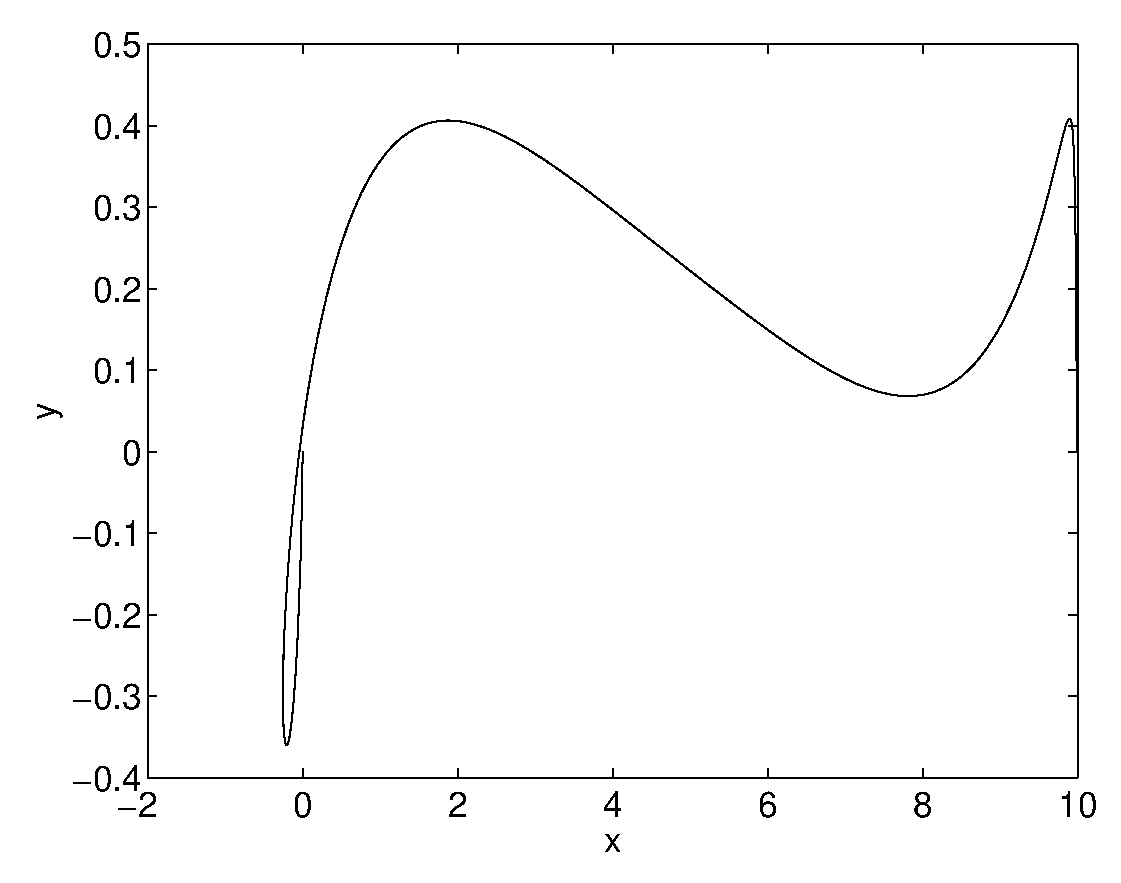
\includegraphics[height=0.3\textheight]{img/final_15_1_10_path.eps}
\caption{path}
\end{subfigure}

\begin{subfigure}[b]{\textwidth}
\centering
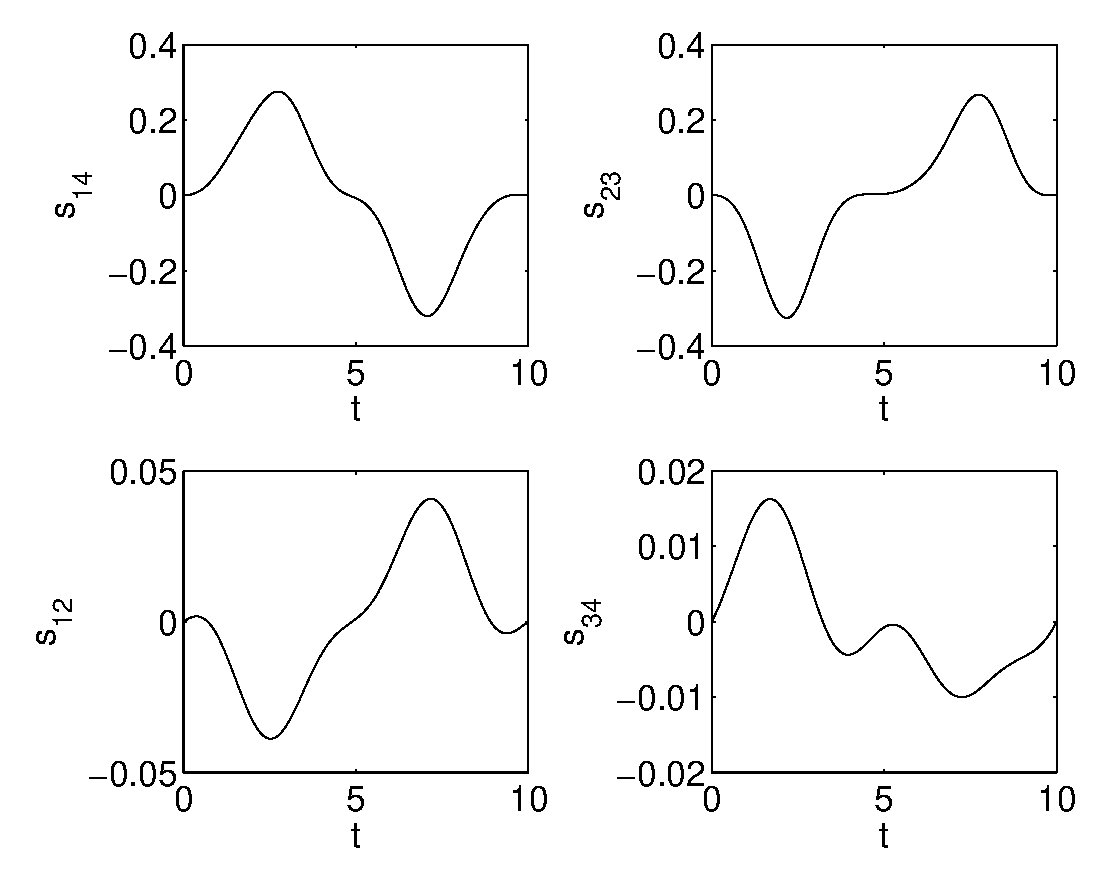
\includegraphics[height=0.3\textheight]{img/final_15_1_10_slips.eps}
\caption{slips}
\end{subfigure}

\begin{subfigure}[b]{\textwidth}
\centering
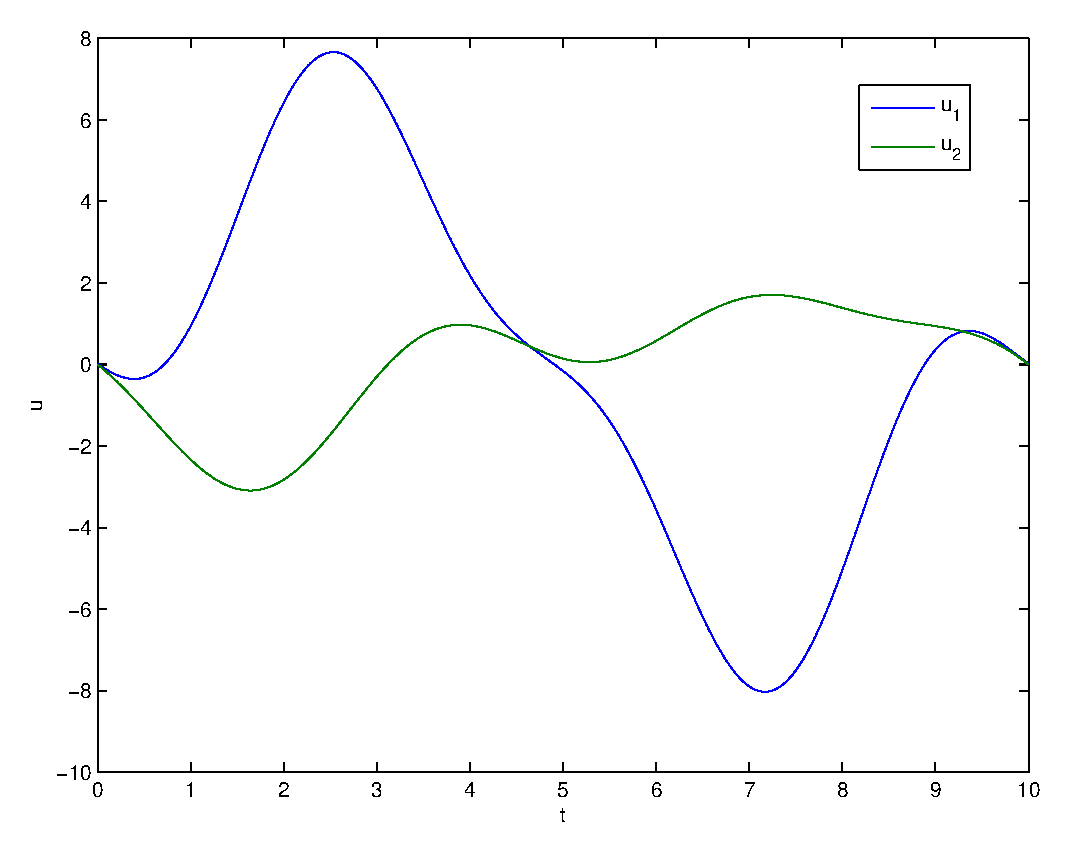
\includegraphics[height=0.3\textheight]{img/final_15_1_10_u.eps}
\caption{path}
\end{subfigure}
\caption{Mobile platform, $\epsilon=15$, $\tau=1$, $T=10$}
\label{fig:pl1}
\end{figure}

\begin{figure}[h]
\begin{subfigure}[b]{\textwidth}
\centering
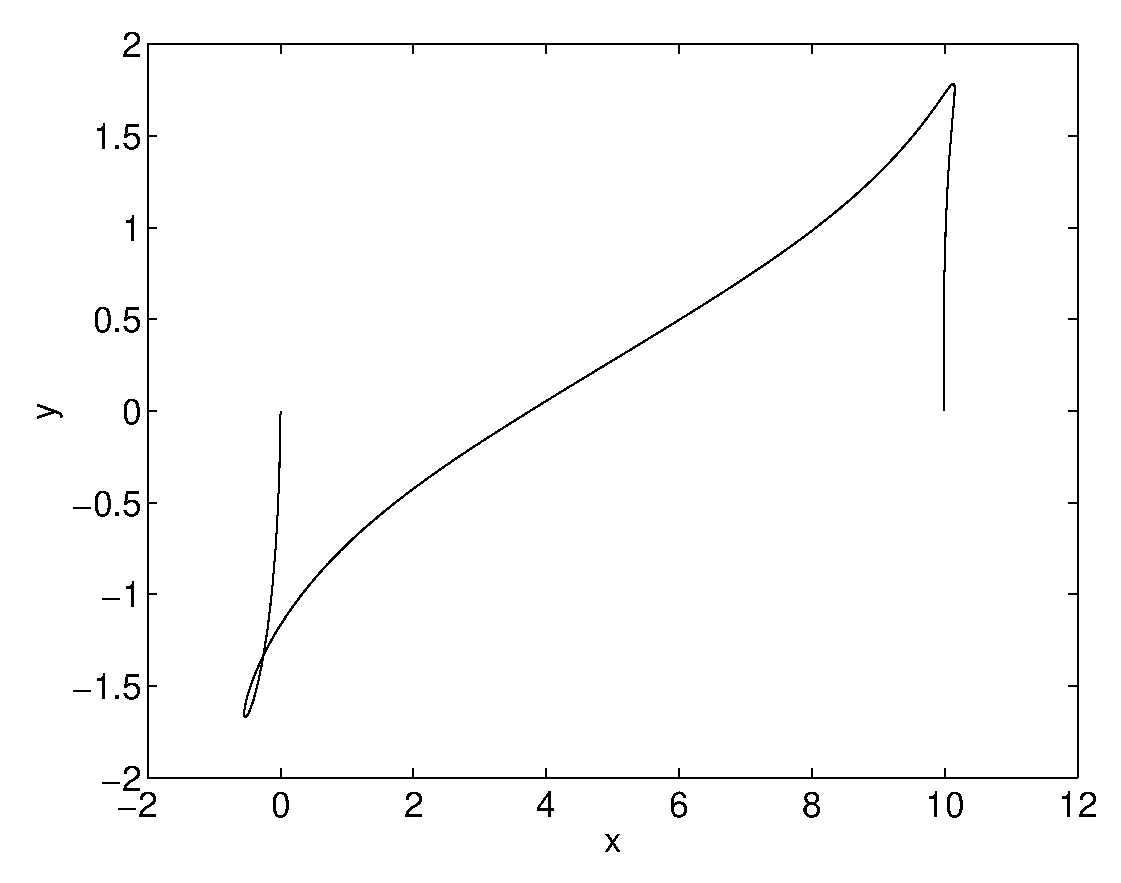
\includegraphics[height=0.3\textheight]{img/final_15_1_20_path.eps}
\caption{path}
\end{subfigure}

\begin{subfigure}[b]{\textwidth}
\centering
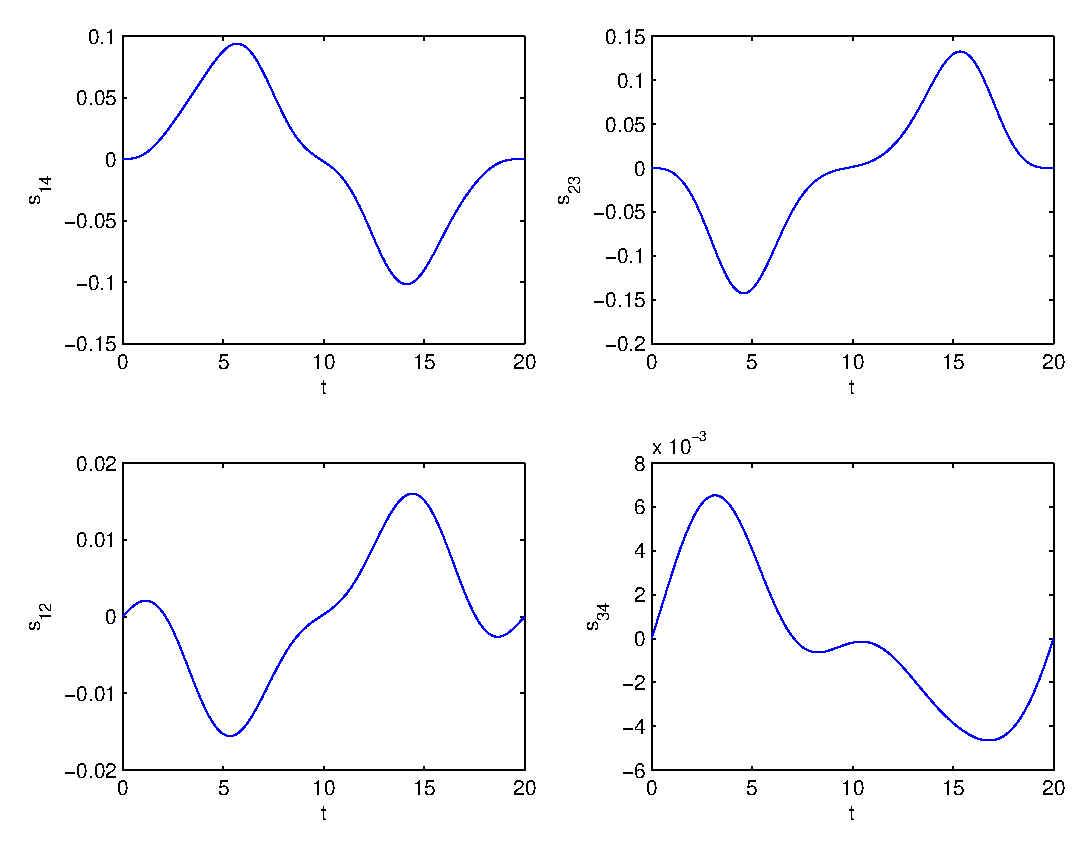
\includegraphics[height=0.3\textheight]{img/final_15_1_20_slips.eps}
\caption{slips}
\end{subfigure}

\begin{subfigure}[b]{\textwidth}
\centering
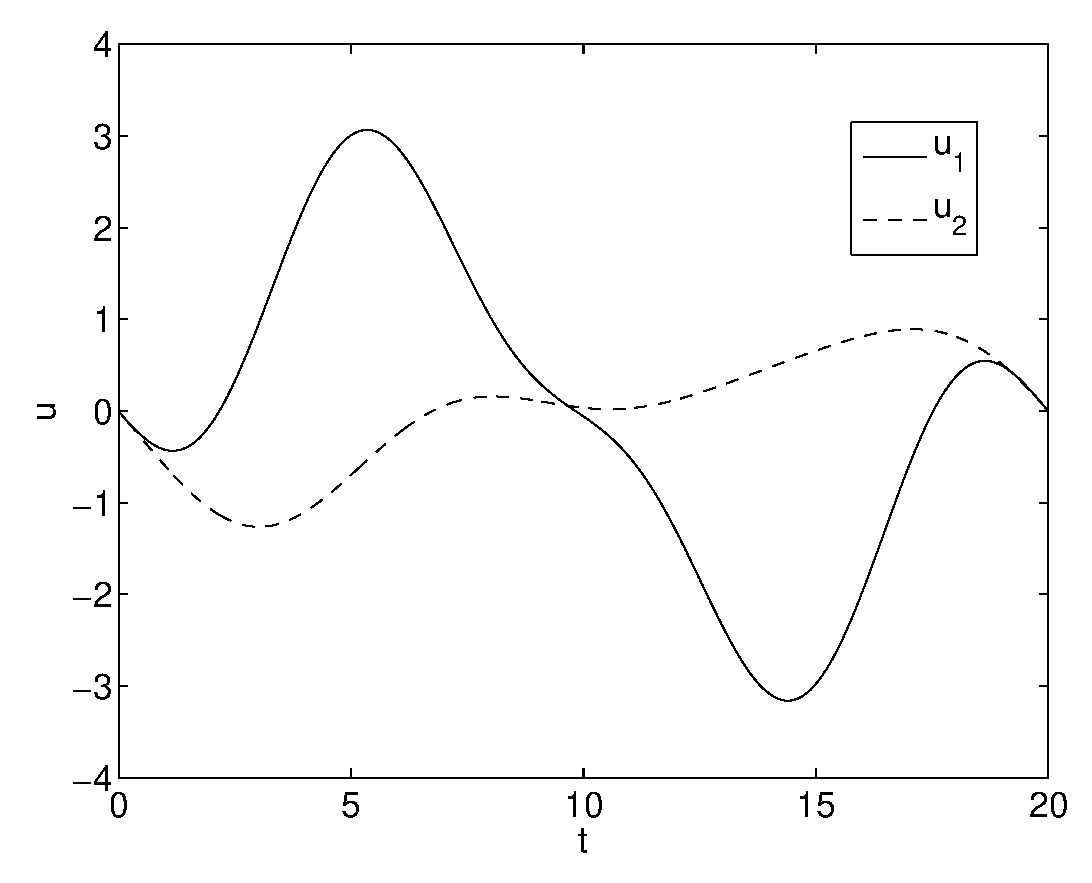
\includegraphics[height=0.3\textheight]{img/final_15_1_20_u.eps}
\caption{path}
\end{subfigure}
\caption{Mobile platform, $\epsilon=15$, $\tau=1$, $T=20$}
\label{fig:pl2}
\end{figure}

%%%%%%%%%%%%%%%%%%%%%%%%%%%%%%%%%%%%%%%%%%%%%%%%%%%%%%%%%%%%%%%%%%%%%%%%%%%%%%%%%%%%%%%%%%%
%%%%%%%%%%%%%%%%%%%%%%%%%%%%%%%%%%%%%%%%%%%%%%%%%%%%%%%%%%%%%%%%%%%%%%%%%%%%%%%%%%%%%%%%%%%
%%%%%%%%%%%%%%%%%%%%%%%%%%%%%%%%%%%%%%%%%%%%%%%%%%%%%%%%%%%%%%%%%%%%%%%%%%%%%%%%%%%%%%%%%%%
%%%%%%%%%%%%%%%%%%%%%%%%%%%%%%%%%%%%%%%%%%%%%%%%%%%%%%%%%%%%%%%%%%%%%%%%%%%%%%%%%%%%%%%%%%%
%%%%%%%%%%%%%%%%%%%%%%%%%%%%%%%%%%%%%%%%%%%%%%%%%%%%%%%%%%%%%%%%%%%%%%%%%%%%%%%%%%%%%%%%%%%

\begin{figure}[h]
\begin{subfigure}[b]{\textwidth}
\centering
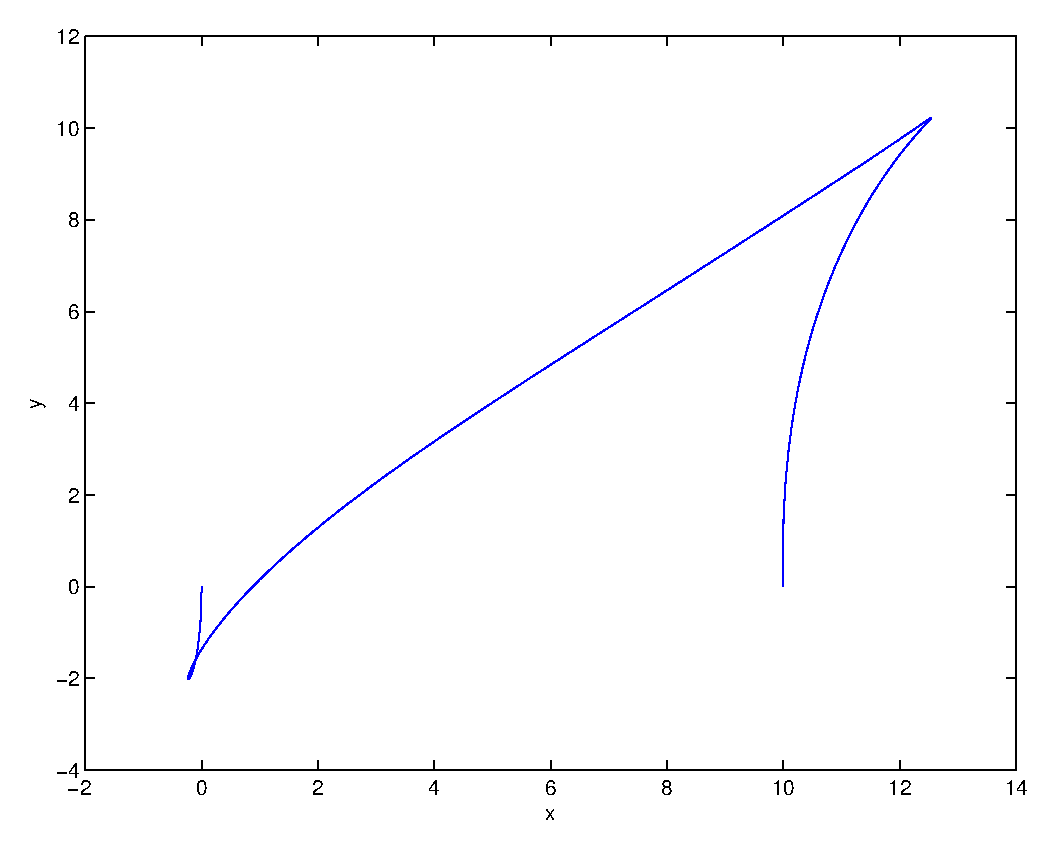
\includegraphics[height=0.3\textheight]{img/final_15_15_10_path.eps}
\caption{path}
\end{subfigure}

\begin{subfigure}[b]{\textwidth}
\centering
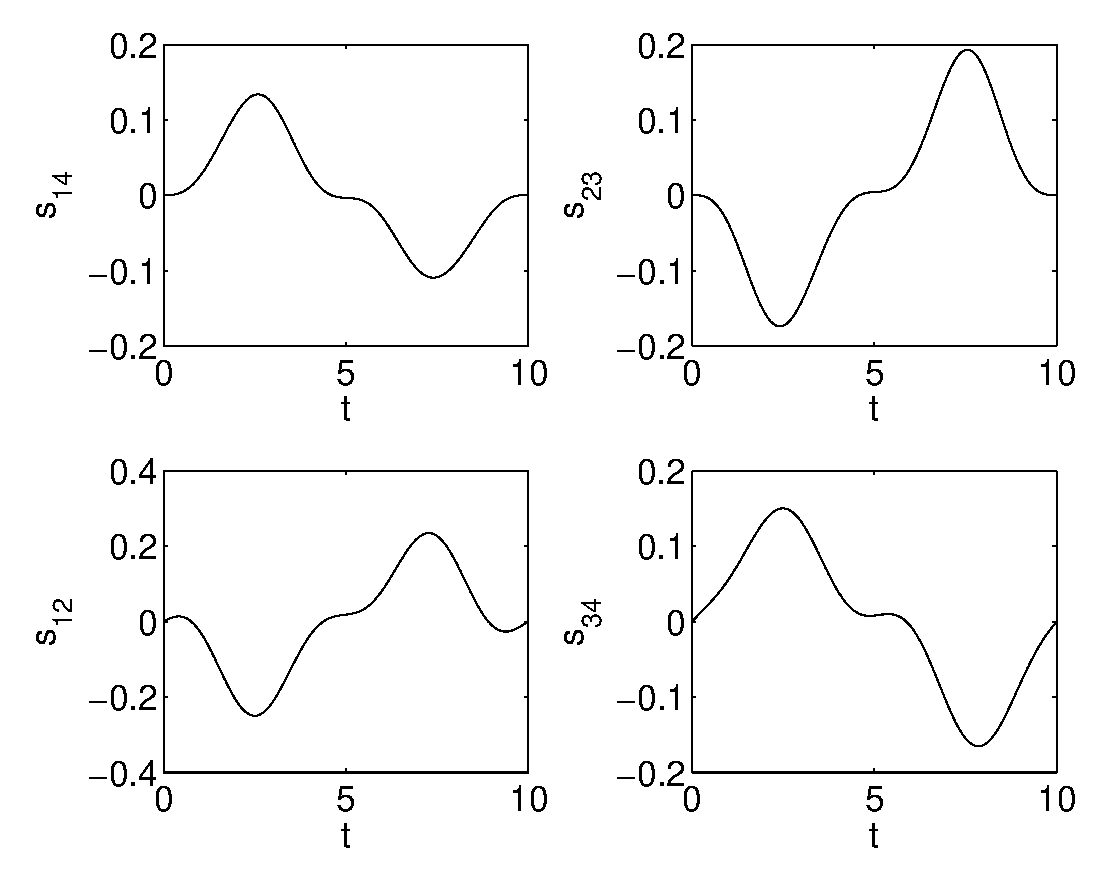
\includegraphics[height=0.3\textheight]{img/final_15_15_10_slips.eps}
\caption{slips}
\end{subfigure}

\begin{subfigure}[b]{\textwidth}
\centering
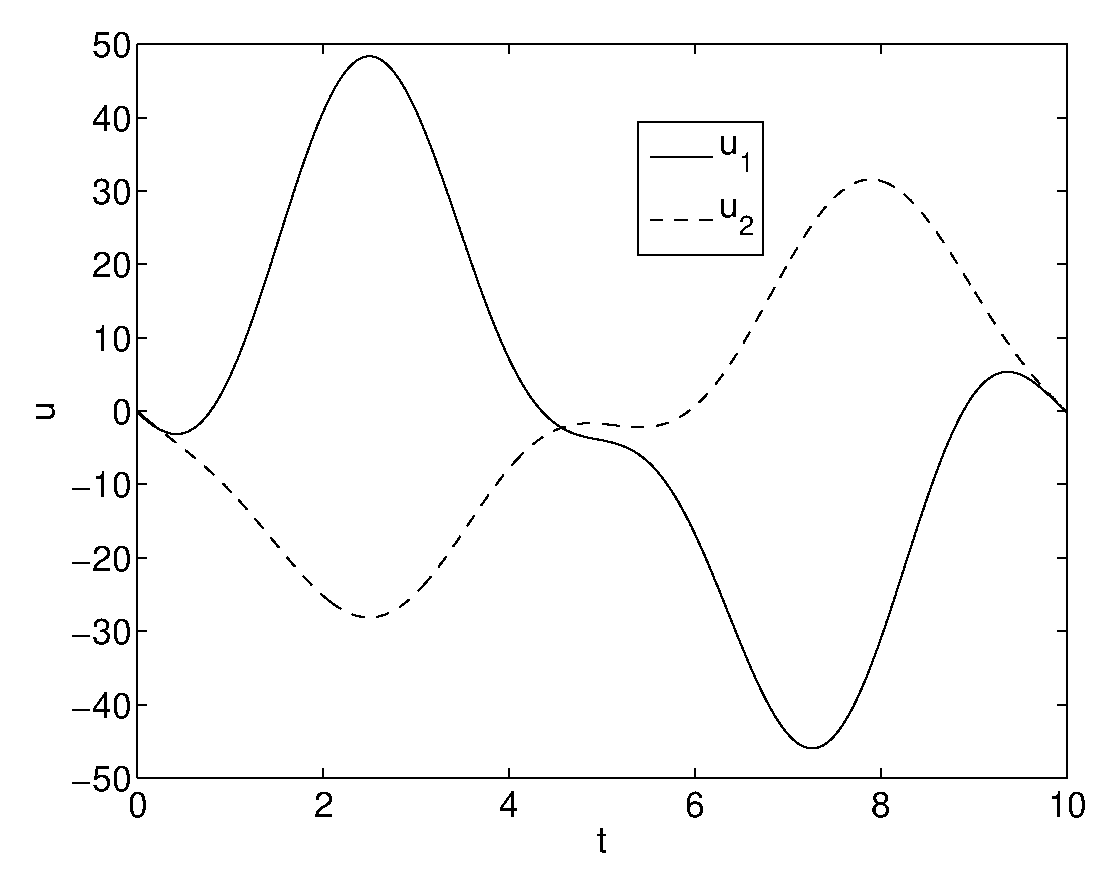
\includegraphics[height=0.3\textheight]{img/final_15_15_10_u.eps}
\caption{path}
\end{subfigure}
\caption{Mobile platform, $\epsilon=15$, $\tau=15$, $T=10$}
\label{fig:pl3}
\end{figure}

\begin{figure}[h]
\begin{subfigure}[b]{\textwidth}
\centering
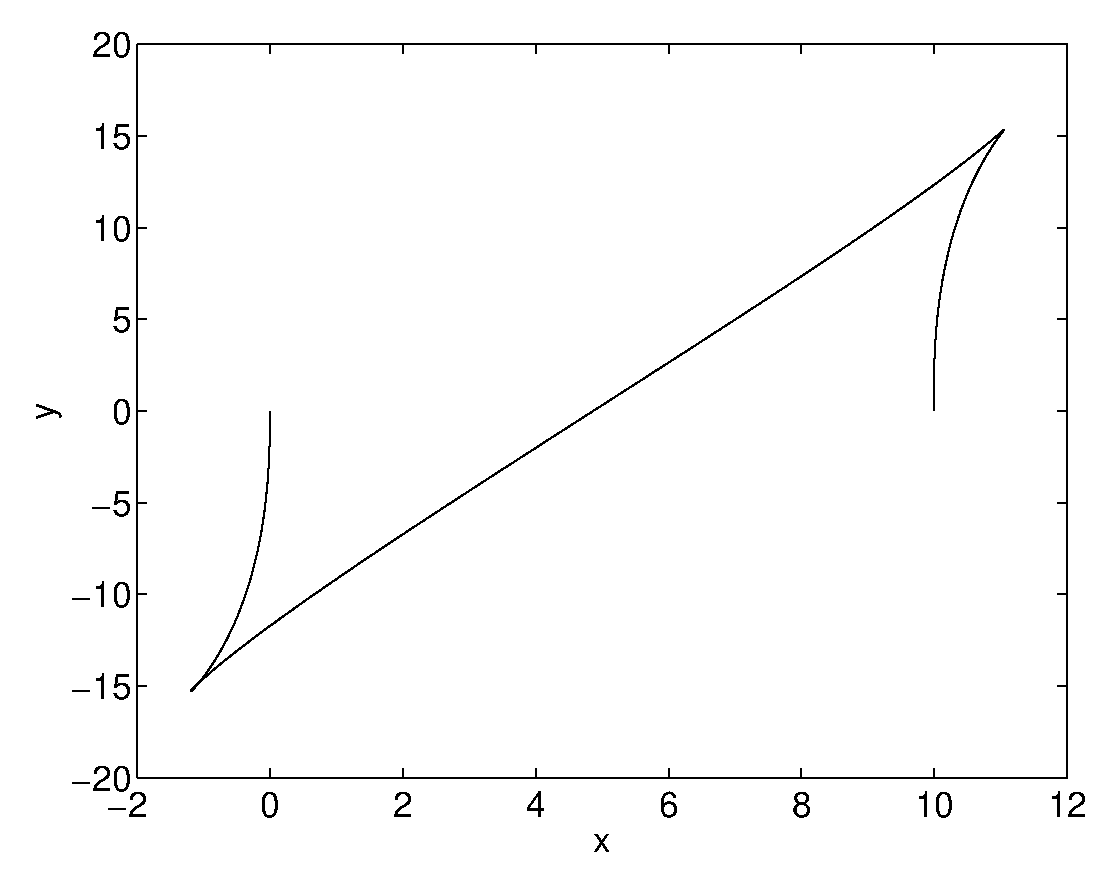
\includegraphics[height=0.3\textheight]{img/final_15_15_20_path.eps}
\caption{path}
\end{subfigure}

\begin{subfigure}[b]{\textwidth}
\centering
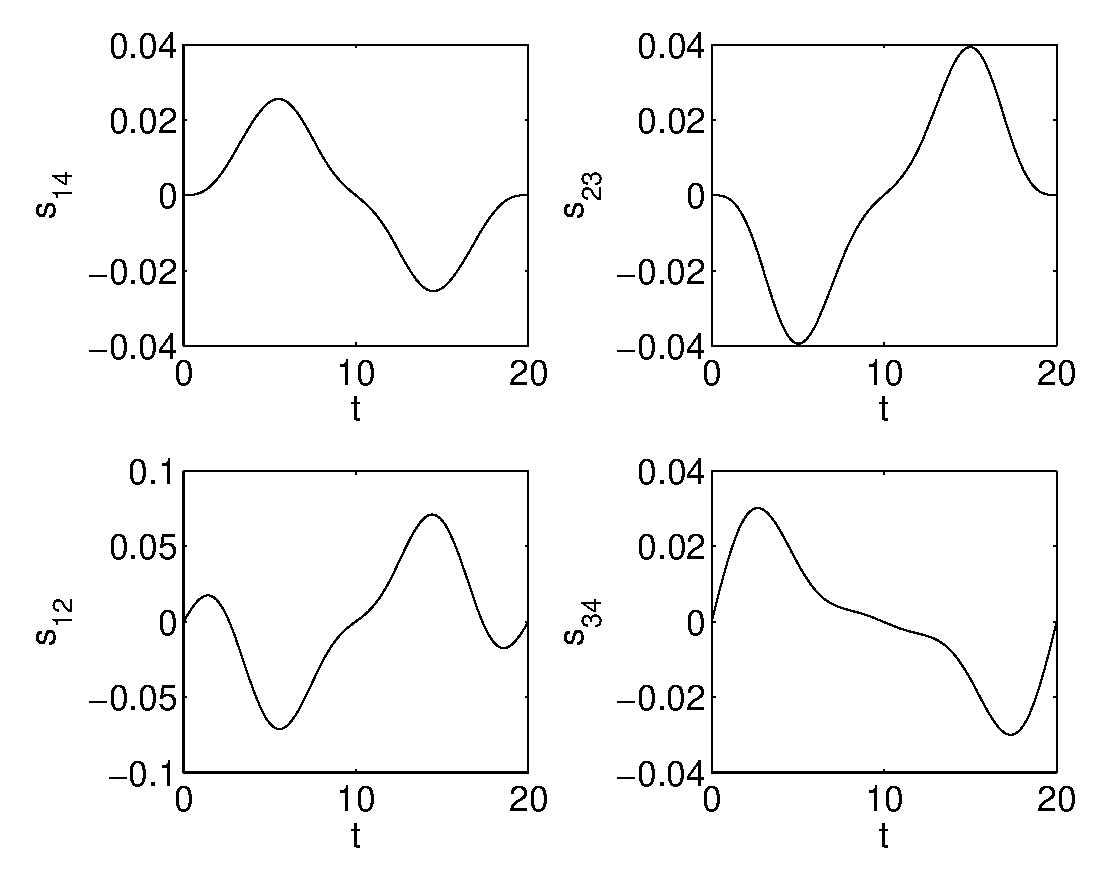
\includegraphics[height=0.3\textheight]{img/final_15_15_20_slips.eps}
\caption{slips}
\end{subfigure}

\begin{subfigure}[b]{\textwidth}
\centering
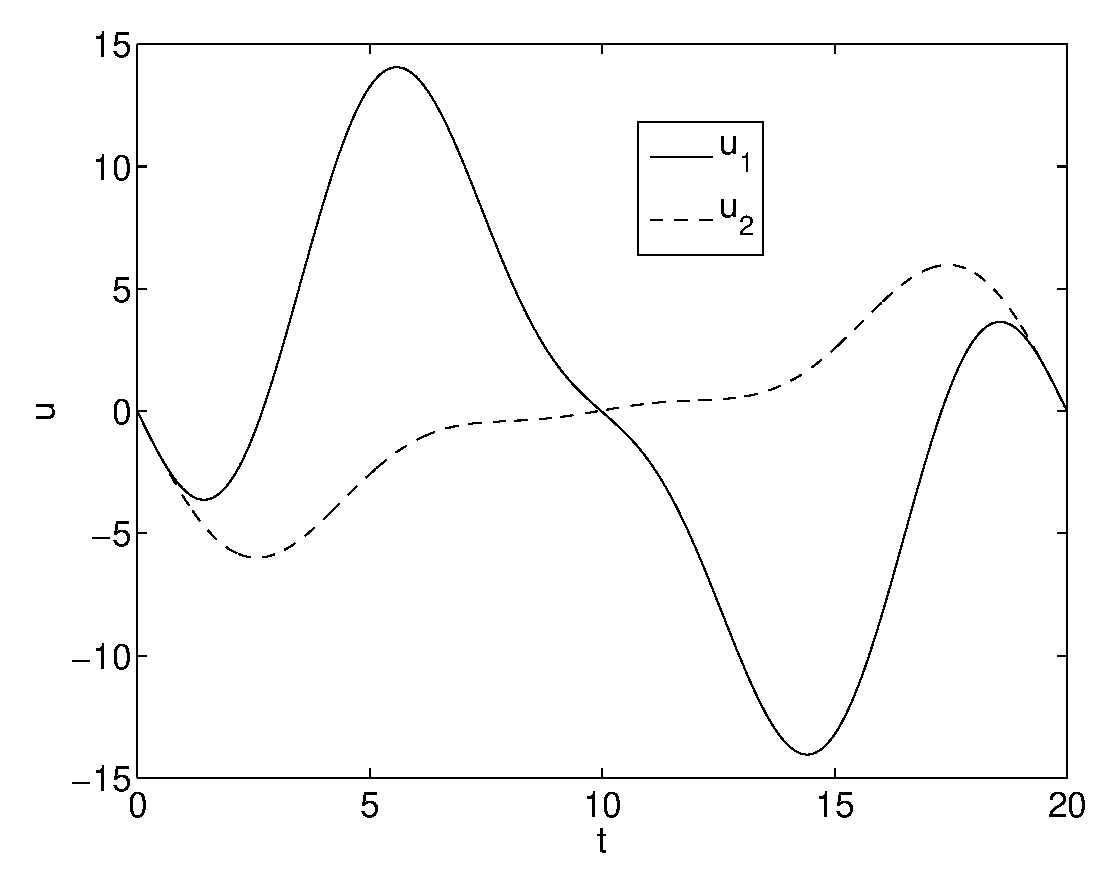
\includegraphics[height=0.3\textheight]{img/final_15_15_20_u.eps}
\caption{path}
\end{subfigure}
\caption{Mobile platform, $\epsilon=15$, $\tau=15$, $T=20$}
\label{fig:pl4}
\end{figure}

%%%%%%%%%%%%%%%%%%%%%%%%%%%%%%%%%%%%%%%%%%%%%%%%%%%%%%%%%%%%%%%%%%%%%%%%%%%%%%%%%%%%%%%%%%%
%%%%%%%%%%%%%%%%%%%%%%%%%%%%%%%%%%%%%%%%%%%%%%%%%%%%%%%%%%%%%%%%%%%%%%%%%%%%%%%%%%%%%%%%%%%
%%%%%%%%%%%%%%%%%%%%%%%%%%%%%%%%%%%%%%%%%%%%%%%%%%%%%%%%%%%%%%%%%%%%%%%%%%%%%%%%%%%%%%%%%%%
%%%%%%%%%%%%%%%%%%%%%%%%%%%%%%%%%%%%%%%%%%%%%%%%%%%%%%%%%%%%%%%%%%%%%%%%%%%%%%%%%%%%%%%%%%%
%%%%%%%%%%%%%%%%%%%%%%%%%%%%%%%%%%%%%%%%%%%%%%%%%%%%%%%%%%%%%%%%%%%%%%%%%%%%%%%%%%%%%%%%%%%
\begin{figure}[h]
\begin{subfigure}[b]{\textwidth}
\centering
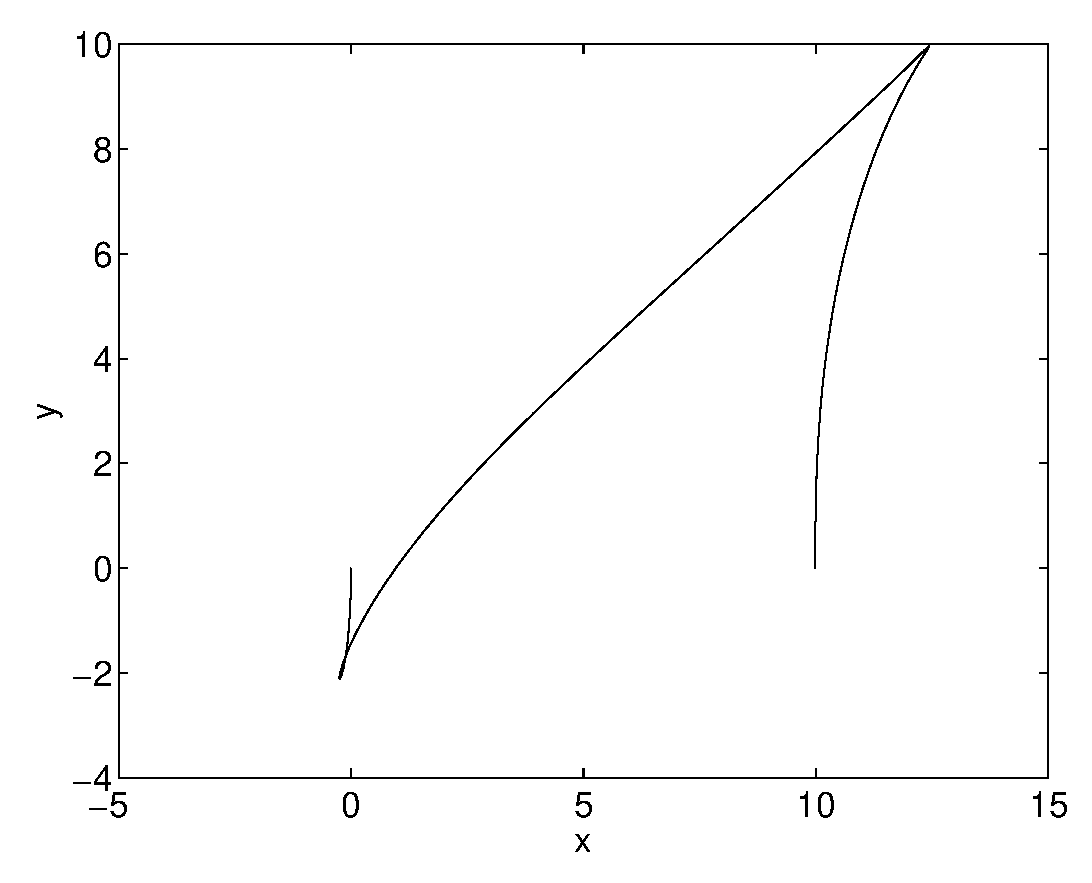
\includegraphics[height=0.3\textheight]{img/final_1_15_10_path.eps}
\caption{path}
\end{subfigure}

\begin{subfigure}[b]{\textwidth}
\centering
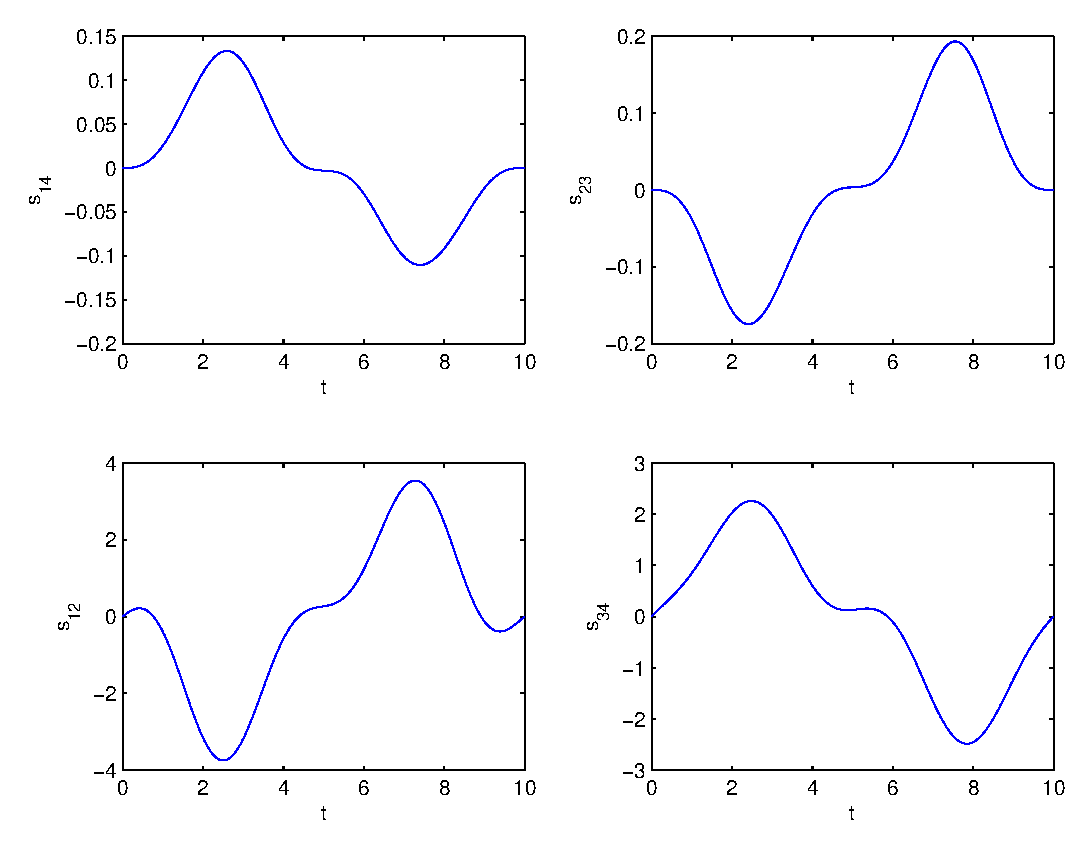
\includegraphics[height=0.3\textheight]{img/final_1_15_10_slips.eps}
\caption{slips}
\end{subfigure}

\begin{subfigure}[b]{\textwidth}
\centering
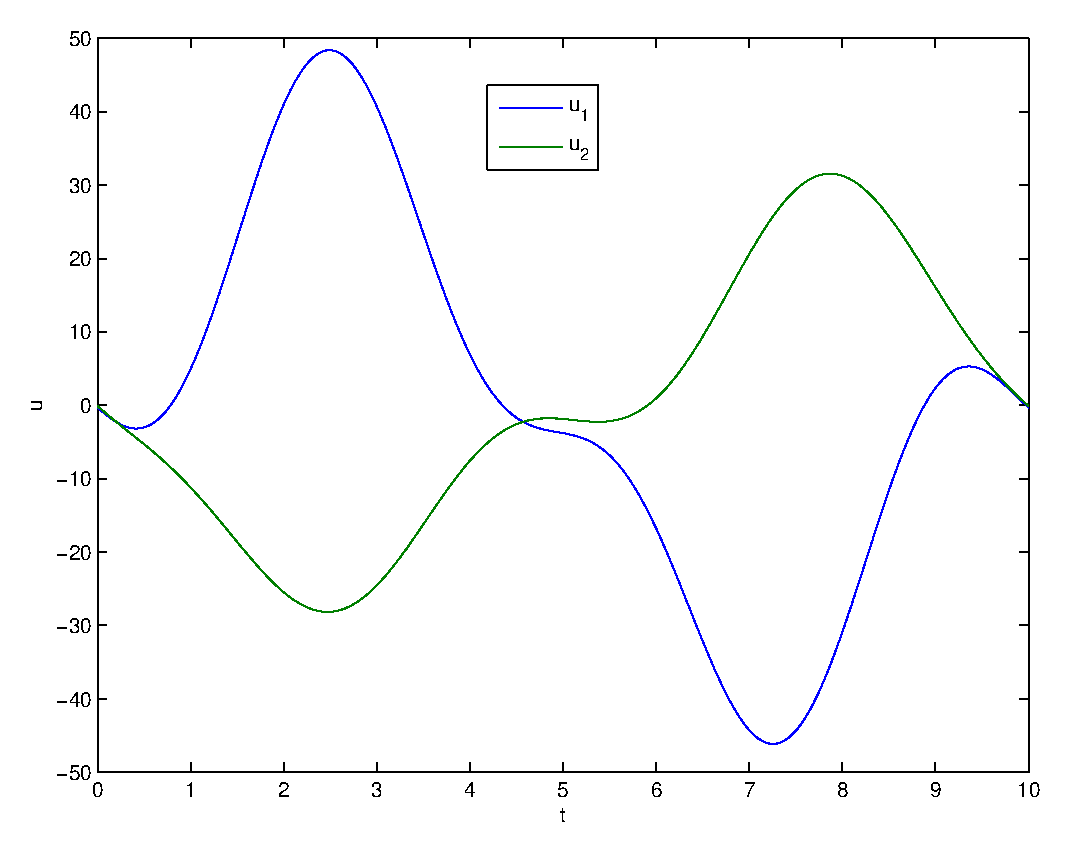
\includegraphics[height=0.3\textheight]{img/final_1_15_10_u.eps}
\caption{path}
\end{subfigure}
\caption{Mobile platform, $\epsilon=1$, $\tau=15$, $T=10$}
\label{fig:pl5}
\end{figure}

\begin{figure}[h]
\begin{subfigure}[b]{\textwidth}
\centering
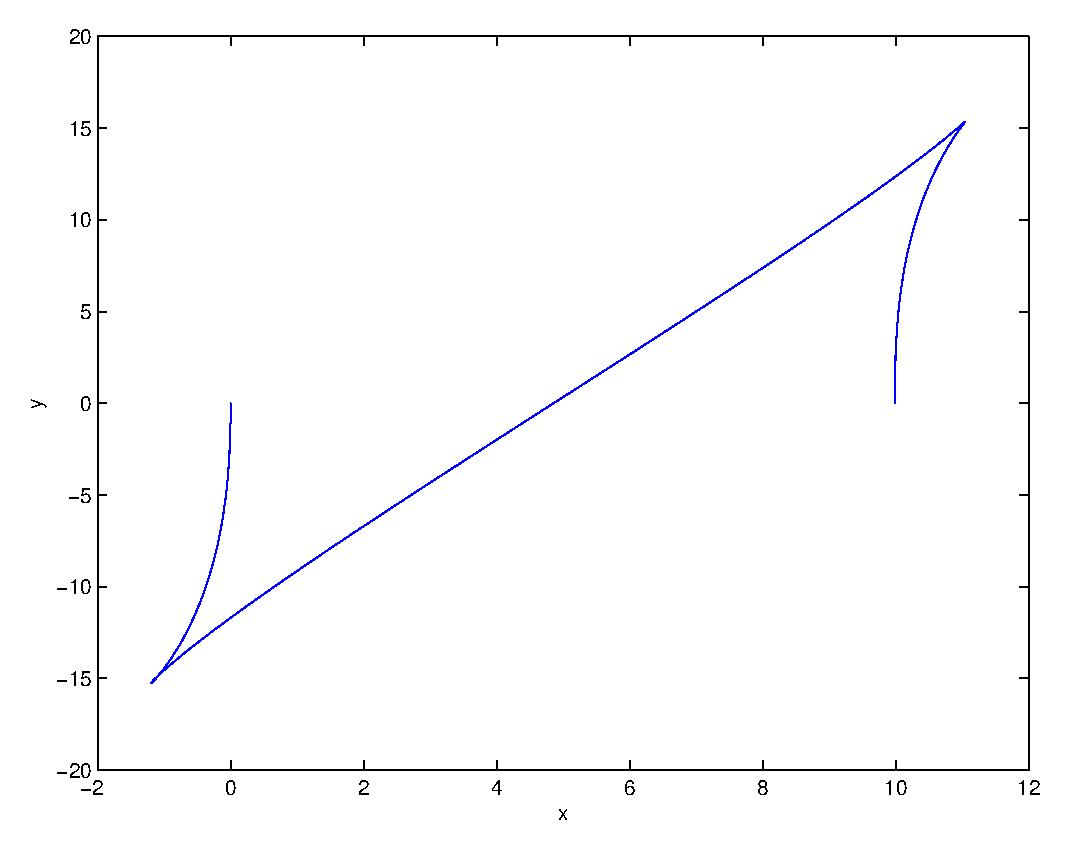
\includegraphics[height=0.3\textheight]{img/final_1_15_20_path.eps}
\caption{path}
\end{subfigure}

\begin{subfigure}[b]{\textwidth}
\centering
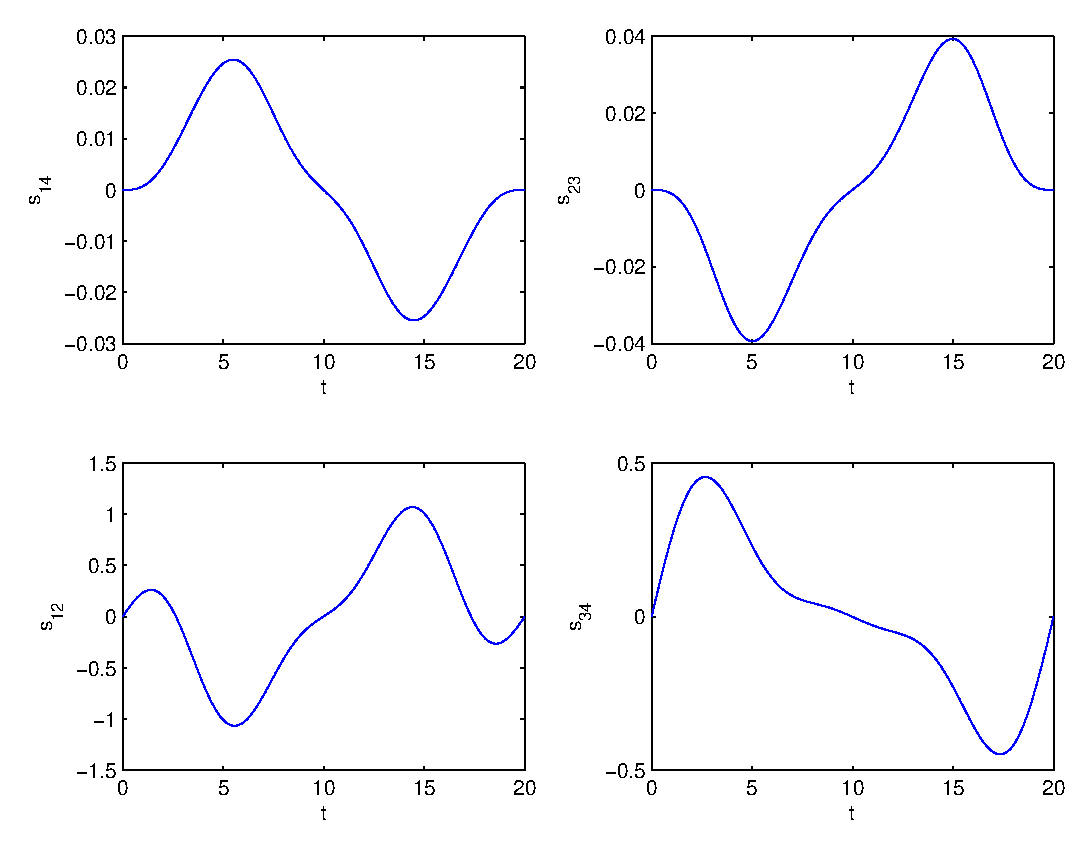
\includegraphics[height=0.3\textheight]{img/final_1_15_20_slips.eps}
\caption{slips}
\end{subfigure}

\begin{subfigure}[b]{\textwidth}
\centering
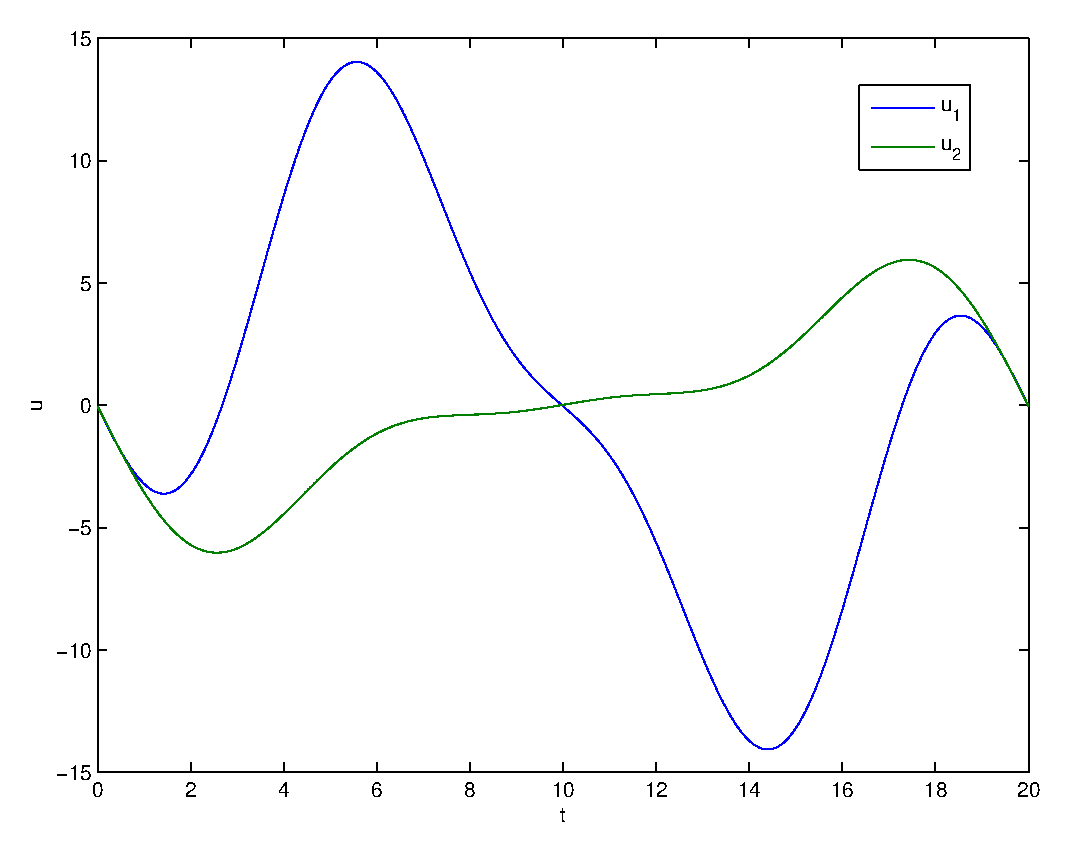
\includegraphics[height=0.3\textheight]{img/final_1_15_20_u.eps}
\caption{path}
\end{subfigure}
\caption{Mobile platform, $\epsilon=1$, $\tau=15$, $T=20$}
\label{fig:pl6}
\end{figure}

%%%%%%%%%%%%%%%%%%%%%%%%%%%%%%%%%%%%%%%%%%%%%%%%%%%%%%%%%%%%%%%%%%%%%%%%%%%%%%%%%%%%%%%%%%%
%%%%%%%%%%%%%%%%%%%%%%%%%%%%%%%%%%%%%%%%%%%%%%%%%%%%%%%%%%%%%%%%%%%%%%%%%%%%%%%%%%%%%%%%%%%
%%%%%%%%%%%%%%%%%%%%%%%%%%%%%%%%%%%%%%%%%%%%%%%%%%%%%%%%%%%%%%%%%%%%%%%%%%%%%%%%%%%%%%%%%%%
%%%%%%%%%%%%%%%%%%%%%%%%%%%%%%%%%%%%%%%%%%%%%%%%%%%%%%%%%%%%%%%%%%%%%%%%%%%%%%%%%%%%%%%%%%%
%%%%%%%%%%%%%%%%%%%%%%%%%%%%%%%%%%%%%%%%%%%%%%%%%%%%%%%%%%%%%%%%%%%%%%%%%%%%%%%%%%%%%%%%%%%
\begin{figure}[h]
\begin{subfigure}[b]{\textwidth}
\centering
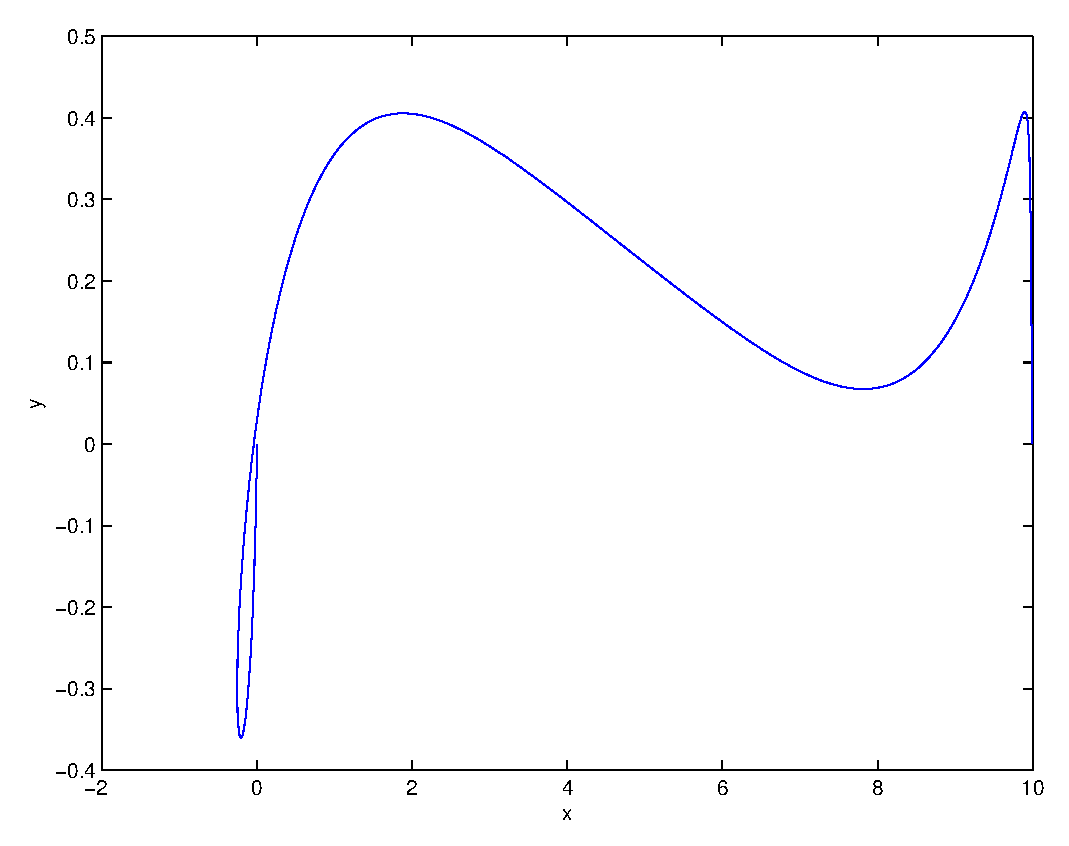
\includegraphics[height=0.3\textheight]{img/final_1_1_10_path.eps}
\caption{path}
\end{subfigure}

\begin{subfigure}[b]{\textwidth}
\centering
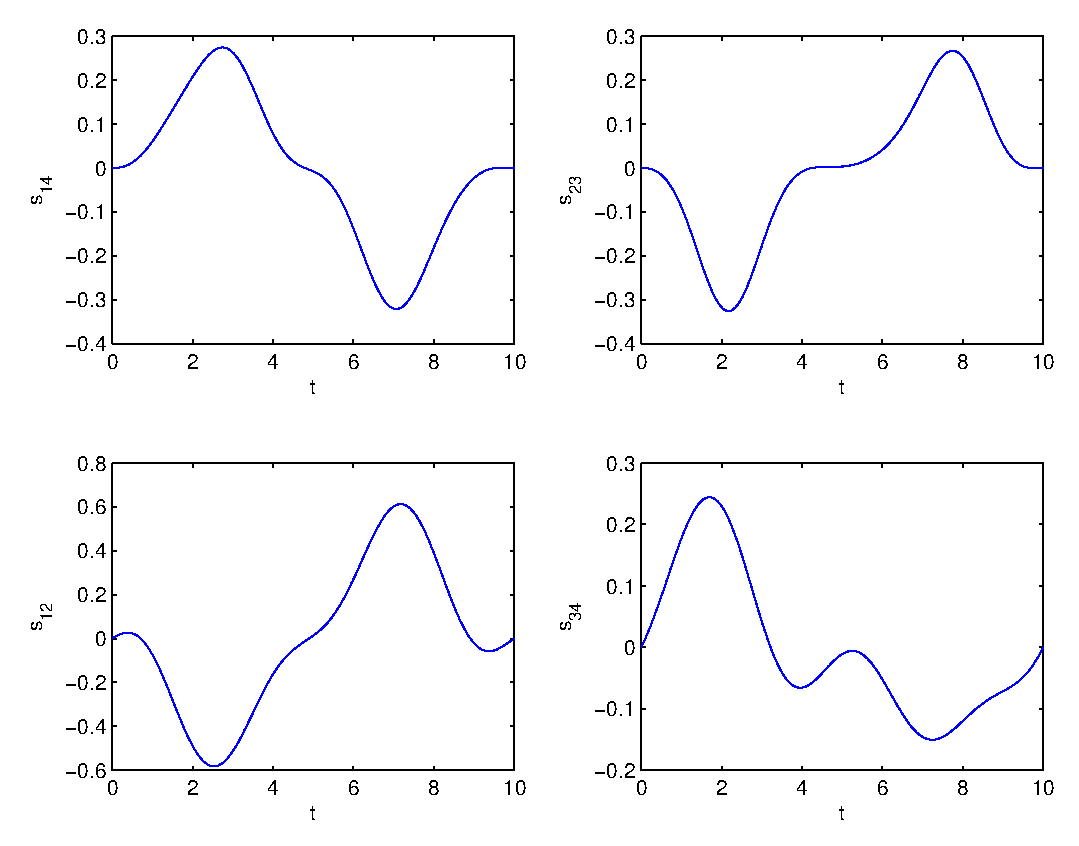
\includegraphics[height=0.3\textheight]{img/final_1_1_10_slips.eps}
\caption{slips}
\end{subfigure}

\begin{subfigure}[b]{\textwidth}
\centering
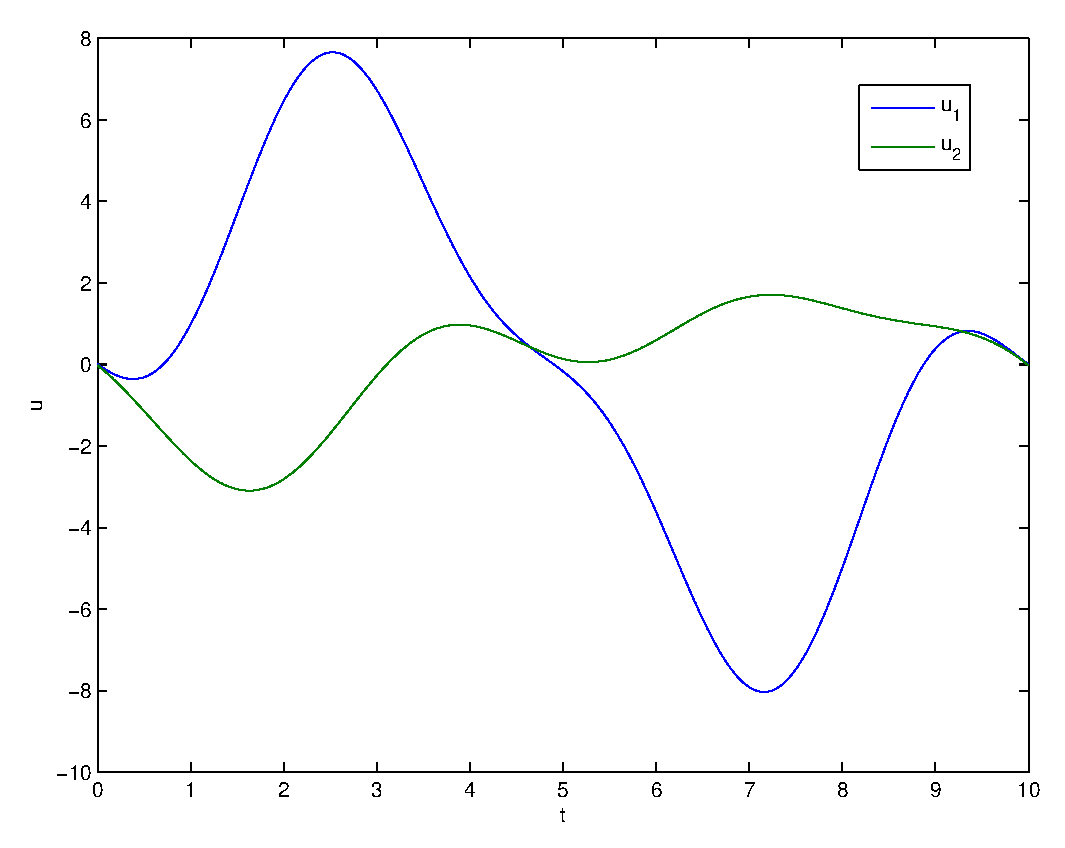
\includegraphics[height=0.3\textheight]{img/final_1_1_10_u.eps}
\caption{path}
\end{subfigure}
\caption{Mobile platform, $\epsilon=1$, $\tau=1$, $T=10$}
\label{fig:pl7}
\end{figure}

\begin{figure}[h]
\begin{subfigure}[b]{\textwidth}
\centering
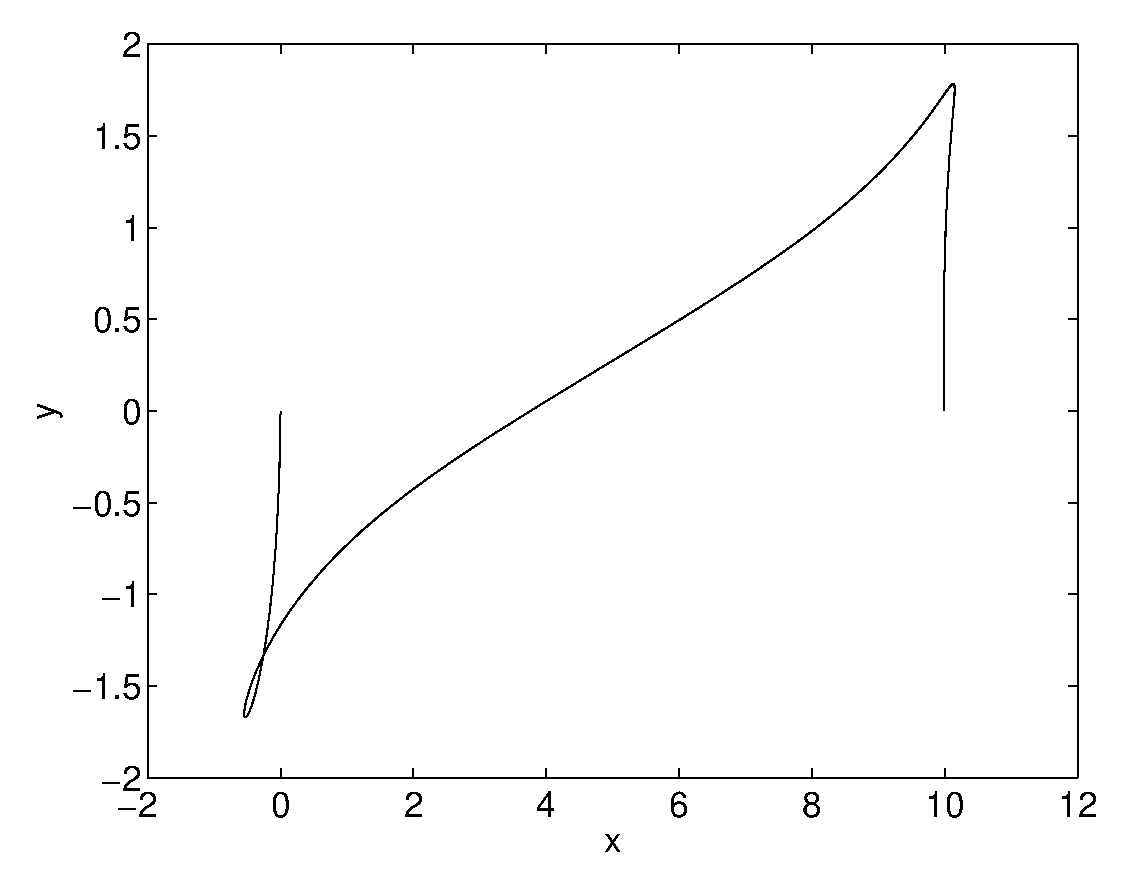
\includegraphics[height=0.3\textheight]{img/final_1_1_20_path.eps}
\caption{path}
\end{subfigure}

\begin{subfigure}[b]{\textwidth}
\centering
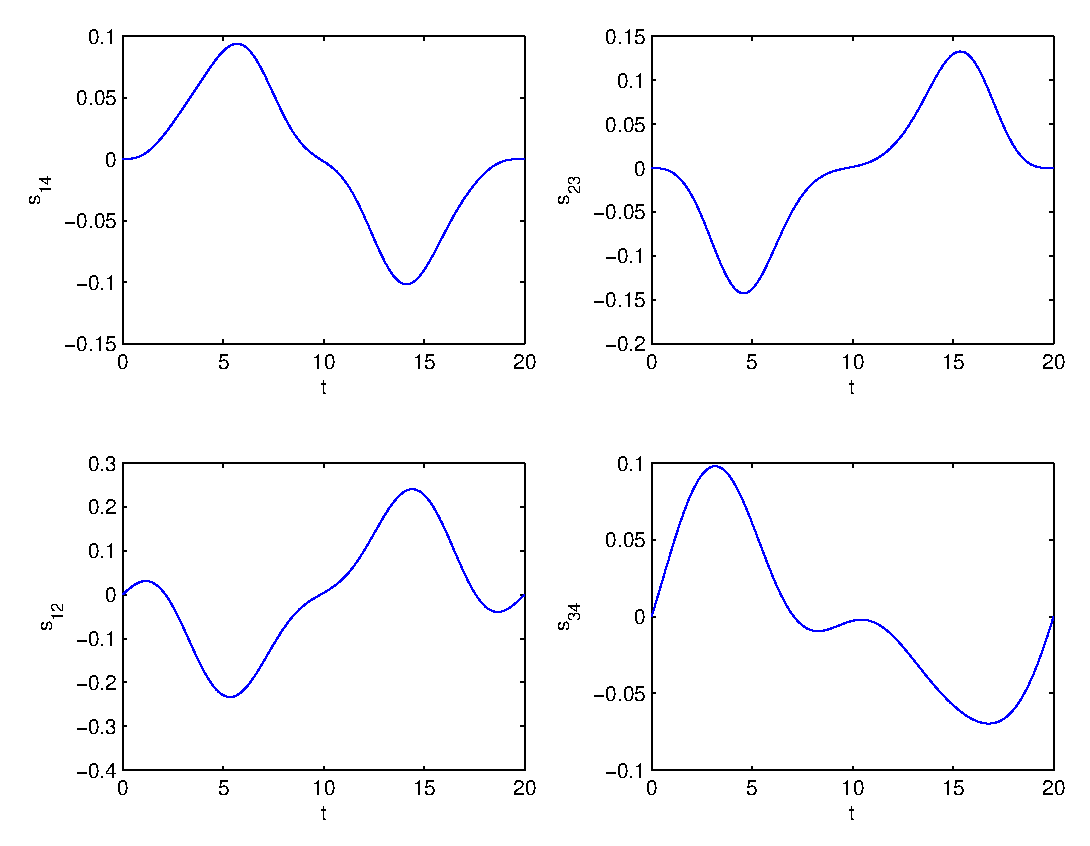
\includegraphics[height=0.3\textheight]{img/final_1_1_20_slips.eps}
\caption{slips}
\end{subfigure}

\begin{subfigure}[b]{\textwidth}
\centering
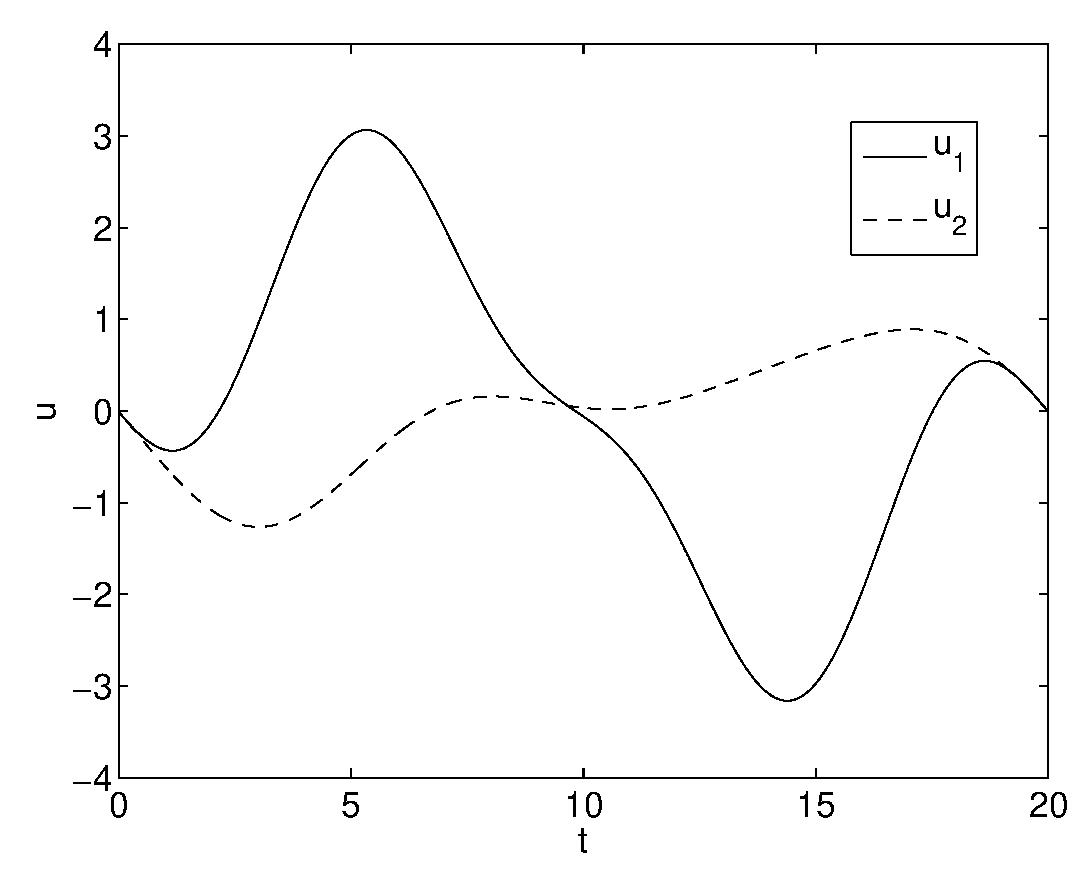
\includegraphics[height=0.3\textheight]{img/final_1_1_20_u.eps}
\caption{path}
\end{subfigure}
\caption{Mobile platform, $\epsilon=1$, $\tau=1$, $T=20$}
\label{fig:pl8}
\end{figure}

%%%%%%%%%%%%%%%%%%%%%%%%%%%%%%%%%%%%%%%%%%%%%%%%%%%%%%%%%%%%%%%%%%%%%%%%%%%%%%%%%%%%%%%%%%%
%%%%%%%%%%%%%%%%%%%%%%%%%%%%%%%%%%%%%%%%%%%%%%%%%%%%%%%%%%%%%%%%%%%%%%%%%%%%%%%%%%%%%%%%%%%
%%%%%%%%%%%%%%%%%%%%%%%%%%%%%%%%%%%%%%%%%%%%%%%%%%%%%%%%%%%%%%%%%%%%%%%%%%%%%%%%%%%%%%%%%%%
%%%%%%%%%%%%%%%%%%%%%%%%%%%%%%%%%%%%%%%%%%%%%%%%%%%%%%%%%%%%%%%%%%%%%%%%%%%%%%%%%%%%%%%%%%%
%%%%%%%%%%%%%%%%%%%%%%%%%%%%%%%%%%%%%%%%%%%%%%%%%%%%%%%%%%%%%%%%%%%%%%%%%%%%%%%%%%%%%%%%%%%

\subsection{Discontinuous friction model}
This model assumes that coefficients $\epsilon_i$ and $\tau_i$ in \eqref{eq:force_r} depend.

\subsection{Manipulator}
When it comes to the manipulator,
its coordinates in task space $(\phi, \theta, \psi, y, z) $ should be equal to
$(-\frac{\pi}{2}, -\frac{\pi}{4}, \frac{\pi}{2}, 0, 0.2)$.
This corresponds to a parking manoeuvre with the manipulator
looking straight forward, observing the floor right in front of it.
\section{Unicycle}